\documentclass[a4paper,11pt]{report}
\usepackage{fixltx2e}
\usepackage{multirow}
\usepackage{graphicx}
\title{Using GPU's to Solve the Sequence Alignment Problem }
\author{Nilesh Kulkarni \and Sushant Hiray \and Ravi Kumar Roshan \and Vipul Harsh}

\begin{document}

\maketitle
\tableofcontents

\begin{abstract}
The purpose of this project is to see the computational capabilitises of the GPU's in comparison to our legendry CPU which was used for all operations in the past. To harness the GPU's power we tried to solve the sequence alignment problem and compare the results between the two paradigms of computing.
\end{abstract}


\chapter{Introduction}
Graphics Processing Units(GPUs) are specialized processors which assist CPUs in rendering graphics by offloading the graphical processing work from the CPUs. Recent advances in the processing capability of GPUs have made them an attractive alternative for performing high performance computations GPUs have a parallel architecture which, until recently, was limited to performing graphical computations. Using GPUs for general purpose computing usually involved rewriting the CPU based algorithm in graphics primitives to enable its evaluation on GPUs. Such an approach requires knowledge of graphics programming and proved to be an hindrance in the adoption of GPUs for general purpose computing. However, with the introduction of CUDA, it has become possible to write algorithms in a familiar programming environment and take full advantage of GPU’s programming capabilities. CUDA is an extension of C language and does not require the knowledge of graphics programming.

In bioinformatics, a sequence alignment is a way of arranging the sequences of DNA, RNA, or protein to identify regions of similarity that may be a consequence of functional, structural, or evolutionary relationships between the sequences. Aligned sequences of nucleotide or amino acid residues are typically represented as rows within a matrix. Gaps are inserted between the residues so that identical or similar characters are aligned in successive columns.

Computational approaches to sequence alignment generally fall into two categories: global alignments and local alignments. Calculating a global alignment is a form of global optimization that "forces" the alignment to span the entire length of all query sequences. By contrast, local alignments identify regions of similarity within long sequences that are often widely divergent overall. Local alignments are often preferable, but can be more difficult to calculate because of the additional challenge of identifying the regions of similarity. A variety of computational algorithms have been applied to the sequence alignment problem. These include slow but formally correct methods like dynamic programming. These also include efficient, heuristic algorithms or probabilistic methods designed for large-scale database search, that do not guarantee to find best matches.

\chapter{CUDA Programming Model}
Compute Unified Device Architecture(CUDA) is a parallel computing architecture developed by
Nvidia to open up Graphics Processing Units(GPUs) to general purpose computing.

\section{Overview}
The GPU acts as a co-processor the CPU (also known as the host) in CUDA. One of the C language
extensions which CUDA provides allows the programmer to specify that a function is to be executed
on the GPU. Such functions are known as kernels and can be called as any other functions from
the main CPU code. The act of calling a kernel is known as a kernel launch. During a kernel
launch, the programmer can specify the number of threads which must be associated with the
current execution of the kernel. Threads are grouped into blocks, with each block having a three
dimensional addressing scheme to identify the threads within each block. The blocks are organized
into a grid which also has a three dimensional addressing scheme to identify the blocks. Every
thread has access to its thread and block identification through inbuilt variables. CUDA also provides a synchronization function which allows all the threads in a block to synchronize at a particular point in the code execution.

\section{Memory Model}
CUDA makes a clear distinction between the RAM accessible from the CPU (called the host
memory) and the RAM available to the GPU (called the device memory). Direct access in not
possible from one type of processor to another.
Within the GPU,each thread has its private set of registers and local memory. All the threads in
a thread block have access to the shared memory of the multiprocessor they are executing on.The
contents of the shared memory are visible to all the threads in the block.

For shared memory, memory access is as fast as accessing registers. This will be true as long
as there are any bank conflicts. The shared memory space is divided into equally sized modules
called banks. During the execution of a warp, if memory access is such that each thread accesses
a different bank in the shared memory, then all memory transfers can happen simultaneously, thus
increasing the memory bandwidth. However, if there are bank conflicts, that is, two or more threads
access the same bank of memory then their access is serialized and memory bandwidth achieved is
not as high as it could be.


\chapter{Global Alignment Problem}

Sequence alignment is the problem of finding regions of similarity between two or more sequences,
typically consisting of nucleotides or amino acids. Global alignment is a type of sequence alignment
where two sequences are aligned with each other with goal of finding similarity between the entire
sequences. If the two sequences are a\textsubscript{1} a\textsubscript{2} ..a\textsubscript{n} and b\textsubscript{1} b\textsubscript{2} ...b\textsubscript{m} , then the final alignment resulting from
global alignment will consist of one character of the first sequence aligned with a character from
the second sequence(a\textsubscript{i} aligned with b\textsubscript{j} ) or a character from either of the sequences aligned with
a gap character(-). The best alignment is chosen based on its alignment score.

There are two ways of dealing with
gaps - Constant Gap Penalty and Affine Gap Penalty. The basic algorithm for solving the global
alignment problem, called the \textbf{\underline{Needleman-Wunsch algorithm}}, is described below.

\section{Constant Gap Penalty}
With every gap alignment is an associated gap penalty(g). For other alignments between two characters, the score
is taken from a substitution matrix, which has a score for every possible character to character
alignment. The best alignment is calculated by using a matrix M of size (n + 1)*(m + 1) where
n and m are the size of the two sequences under consideration.
The cell M(i, j) in the i\textsuperscript{th} row and j\textsuperscript{th} column denotes the best of possible alignment of the two prefixes, obtained from the first
and second sequences respectively, that is, if the two sequences are a\textsubscript{1} a\textsubscript{2} ..a\textsubscript{n} and b\textsubscript{1} b\textsubscript{2} ...b\textsubscript{m} then the cell denotes the best possible alignment of a\textsubscript{1} a\textsubscript{2} ..a\textsubscript{(i-1)} and b\textsubscript{1} b\textsubscript{2} ...b\textsubscript{(j-1)} .

The matrix is filled up using a dynamic programming algorithm as described in the
Needleman-Wunsch Algorithm. For calculating the value in the cell M (i, j) of the matrix there are
three subcases -
\begin{itemize}
  \item  a\textsubscript{i} and b\textsubscript{j} are aligned with each other. It maybe possible that both the characters are same or different. The penalty imposed is usually based on the characters present at the locations and is given in
the substitution matrix. \newline
M (i, j) = M (i - 1, j - 1) + sbt(a\textsubscript{(i-1)} , b\textsubscript{(j-1)} )
\item a\textsubscript{i} is aligned with a gap in the second sequence. This case can also be termed as deletion. \newline
M (i, j) = M (i - 1, j) + g  \newline
where g is the gap penalty. Unlike sbt(a\textsubscript{i} , b\textsubscript{j} ), this is equal for all characters in the constant gap case.
\item b\textsubscript{j} is matched with a gap in the first sequence. This case can also be terned as insertion. \newline
M (i, j) = M (i, j - 1) + g
\end{itemize}

The score assigned to M (i, j) is the minimum of the previous three values.From the above description, it can be seen that to calculate the value of an element, we need three
values - two in the previous row and one in the same row. This is shown in figure 3.1.\begin{figure}
  \begin{center}
    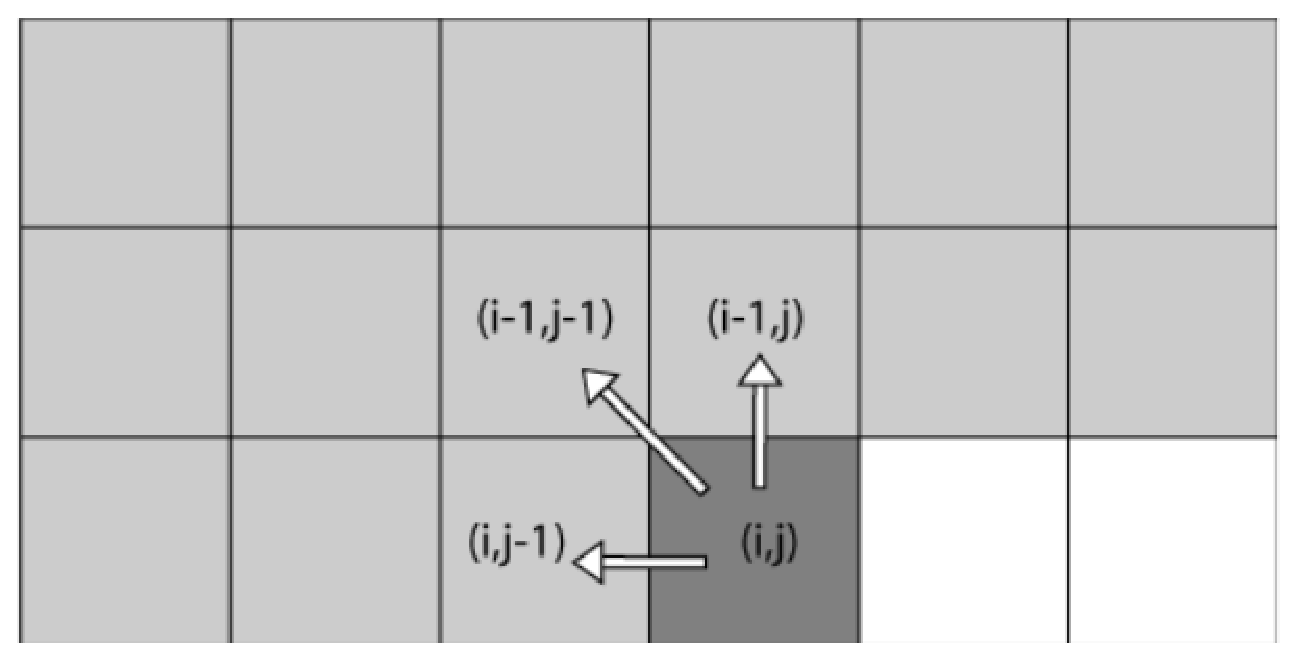
\includegraphics[width=10cm]{fig1}
    \caption{Dependence of cell value on previous cells}
    \label{fig:}
  \end{center}
\end{figure}

The time and space complexity of this algorithm are both quadratic. While the time complexity
can’t be reduced, the space complexity can be reduced to linear space by applying Hirschberg’s
space saving technique without increasing the time complexity.
Due to its quadratic time complexity, we need a faster algorithm for sequences which are of order 1 million long, so as to use them in real world analysis.
In the next chapter we look into a parallel algorithm for solving the problem of sequence alignment which can be implemented on CUDA.
\chapter{Implementation: Parallel Evaluation}
There are two basic approaches to parallel evaluation of the dynamic programming table. We take
a look at the diagonal based approach proposed by Edmiston et. al.  and the parallel prefix based
method proposed by Aluru et. al. .
\section{Diagonal Based Approach}
Conventional evaluation of the dynamic programming table evaluates it row wise (or column wise).
Edmiston et. al.  observed that every element on the diagonal (or more specifically, the an-
tidiagonal) can be evaluated independently of each other. This idea is depicted in Figure 4.1.
The blocks have the same property as the individual elements, that is, blocks on an antidiagonal can be evaluated
independently of each other. \begin{figure}
  \begin{center}
    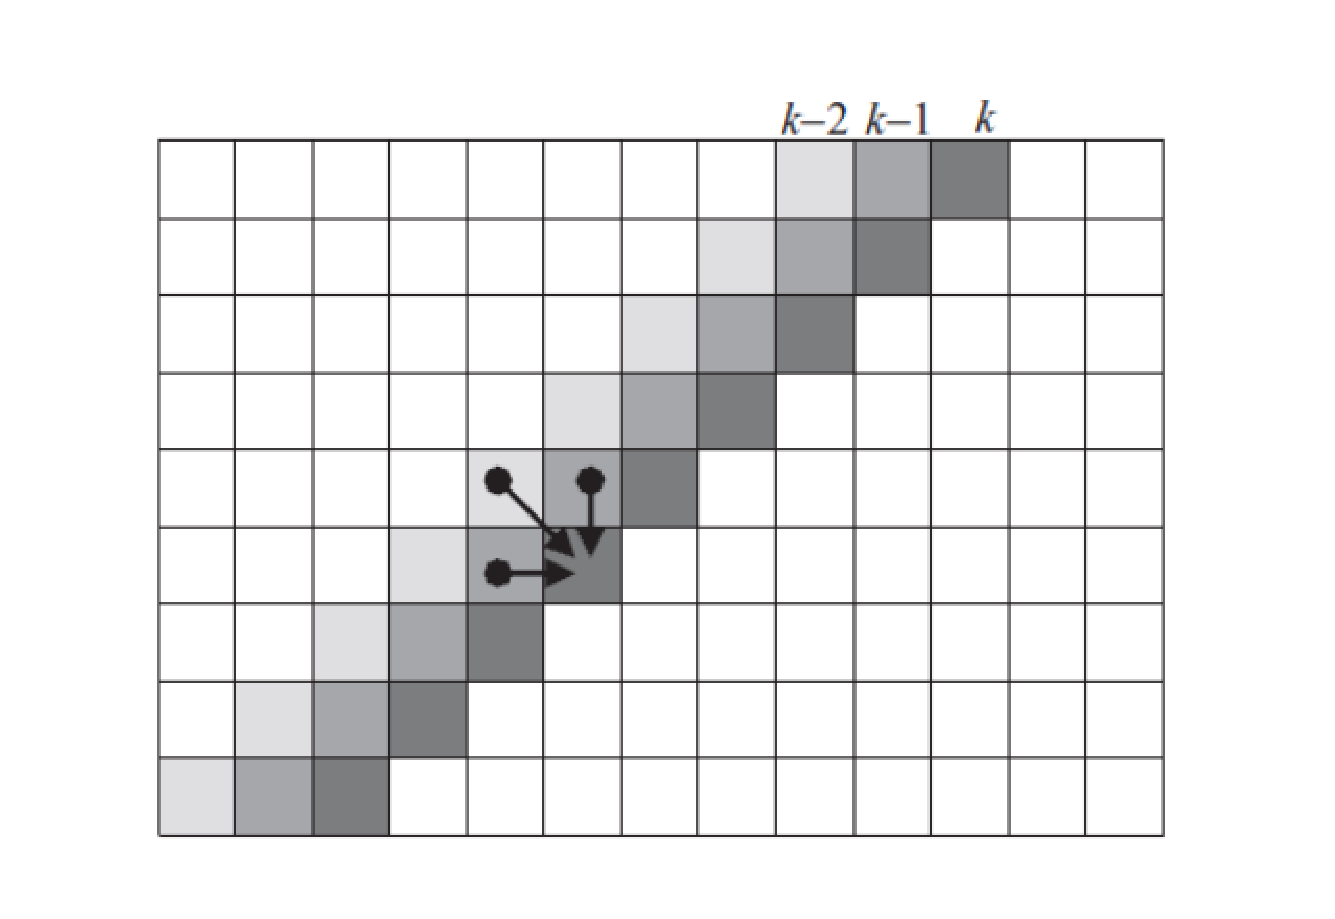
\includegraphics[width=10cm]{fig2}
    \caption{Diagonal Evaluation of Dynamic Programming Table}
    \label{fig:}
  \end{center}
\end{figure}

In the computation stage, all blocks on an antidigaonal are evaluated by
assigning them to different processors. In the communication stage, the processors communicate
their calculated values to those processors which will need in the next stage of computation. Thus,
the technique effectively maintains a wavefront, with the current computation being done on the
edge of the wavefront.
The space complexity of this algorithm is quadratic and is linear in time which is a significant improvement over the sequential dynamic counterpart.



\section{Parallel Prefix Approach}
As mentioned earlier , conventional algorithms evaluate the table row wise. Each row take linear amount of time, summing all of them we obtain an algorithm which runs in quadratic time. The computation of a row can however be made faster( even though the computations are not independent) by employing a tricky Algorithm called the Parallel Prefix method. This method allows to compute each row in logarithmic time resulting in an overall 
$(nlogn$) time. \\

To understand the approach , first consider a simpler version of the problem . We will later abstract it a bit to obtain what we want. \\

Input Array :  $\{x_{1},x_{2},.............x_{2n}\}$  \\

Output Array :   $\{y_{1},y_{2},.............y_{2n}\}$ \\


Where , $y_{i}$  = $\{x_{1} + x_{2}+........  x_{i}\}$  \\


Next , sum up $x_{1}$ and $x_{2}$  , $x_{3}$ and $x_{4}$ ... and so on ,
and we are left with an array of size n.
 $\{v_{1},v_{2}.......................v{n}\}$. \\
 where $\{v_{i} = x_{2i} + x_{2i+1}\}$\\
 
 
 Suppose Recursively we have , the answer for this new array , that is we have  $\{w_{1},v_{2}.......................w{n}\}$. \\
 where  $w_{i}$ = $v_{1}$ + $v_{2}$ ..... $v_{i}$ \\.
 
 
 Observe that now , $y_{2i-1}$ = $w_{i}$  \\
             and ,  $y_{2i}$ = ${w_{i-1}$ + $x_{2i}$.\\
             
             
             
  This can be computed parallely in constant time. There are overall logn levels and thus the algorithm takes logarithmic time.          
                
\chapter{Observations and Inferences}
\section{GPU vs CPU Runtime}
\textbf{Experimental Setup}: \begin{itemize}
  \item Graphics Card: NVIDIA 540M
  \item CPU Intel Processor core i5
  \item 1024 Blocks, 512 Threads
\end{itemize}

We analyse the time taken by both the algorithms (namely sequential dynamic and its parallel counterpart) over a different length of sequences. The following table illustrates the observations:
\begin{table}[ht]
\caption{Running Time Comparison b/w CPU and GPU algorithm} % title of Table
\centering 
\begin{tabular} {| c | c | c | }
\hline
String Length(characters) & CPU Time & GPU Time(Diagonal Approach) \\ \hline
1800 & 00.27s & 01.7s\\
3600 & 00.87s & 03.0s\\ 
4000 & 00.94s & 03.3s\\
7200 & 03.15s & 05.8s \\
8000 & 03.97s & 06.6s \\
14400 & 12.08s & 13.2s \\
16000 & 15.00s & 15.2s \\
17000 & 17.00s & 16.8s \\
17500 & 18.00s & 17.3s \\
\hline
\end{tabular}
\end{table}

\begin{figure}[ht]
  \begin{center}
    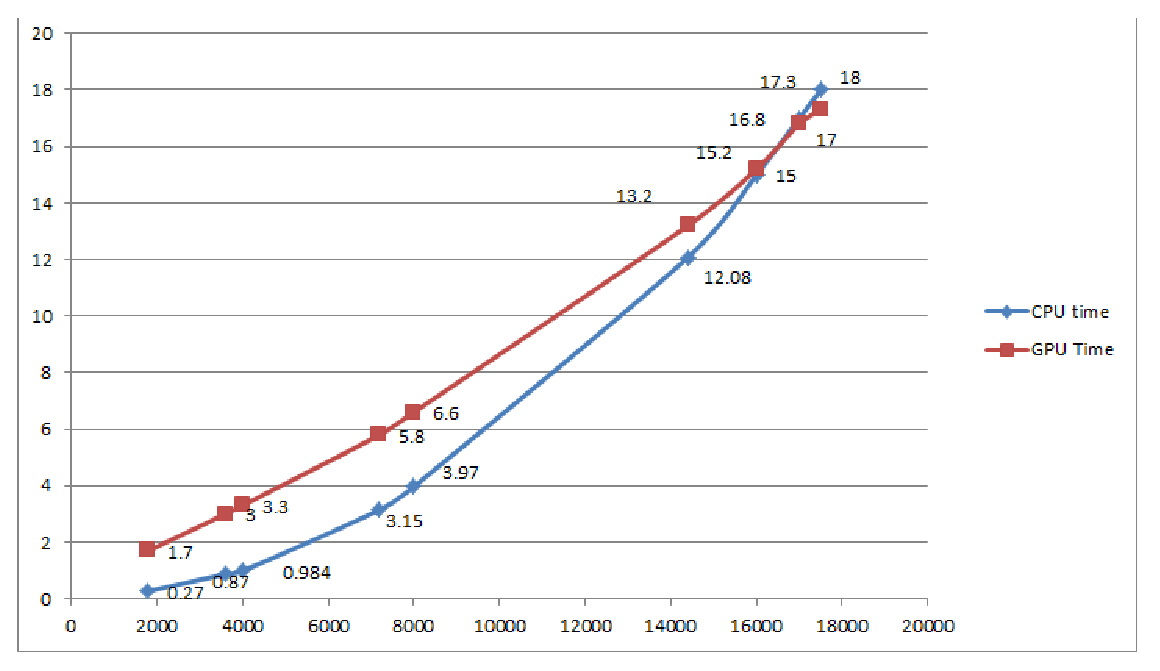
\includegraphics[width=15cm]{gpuvscpu}
    \caption{GPU vs CPU time analysis}
    \label{fig:}
  \end{center}
\end{figure}

We observe that the time taken by CPU is quadratic in nature wheras the time taken by GPU is linear in nature. The nature of the plots can be checked in the figure 5.1.

As can be seen from the data, initially GPU lags considerably in performance as compared to that of CPU but as we increase the size of input data, the performance of GPU improves.

The initial low performance of GPU can be explained by the initial overhead to launch the program. This overhead is due to launching of a GPU kernel from the host, which takes considerable time as compared to that of the normal computation time.

\section{Profiling GPU time}

\begin{table}[ht]
\caption{Running Time Comparison b/w CPU and GPU algorithm} % title of Table
\centering 
\begin{tabular} {| p{2cm} | p{2cm} | p{3cm} | p{2cm} | p{3cm}|}
\hline
String Length & Total Time(s) & CPU Main Fn Time(\%) & Launch Prog Time (\%) & Kernel Function Time(\%)  \\ \hline 
100 & 0.721 & 1.17 & 98.57 & 00.1 \\
1000 & 1.3 & 1.31 & 97.63 & 00.7 \\ 
3000 & 2.6 & 1.21 & 88.31 & 09.6 \\
5000 & 4.3 & 0.73 & 56.86 & 40.4 \\
10000 & 8.5 & 0.51 & 29.38 & 68.1 \\
12700 & 11.3 & 0.32 & 22.2 & 74.2 \\
\hline
\end{tabular}
\end{table}

\section{General Remarks}
These are the general observations found during the execution of the application and analysed using CUDA profiler.
\subsection{Overall Utilisation}
The utilisation levels indicate that the performance of the kernel is most likely being limited by the memory bandwidth.
\begin{figure}
  \begin{center}
    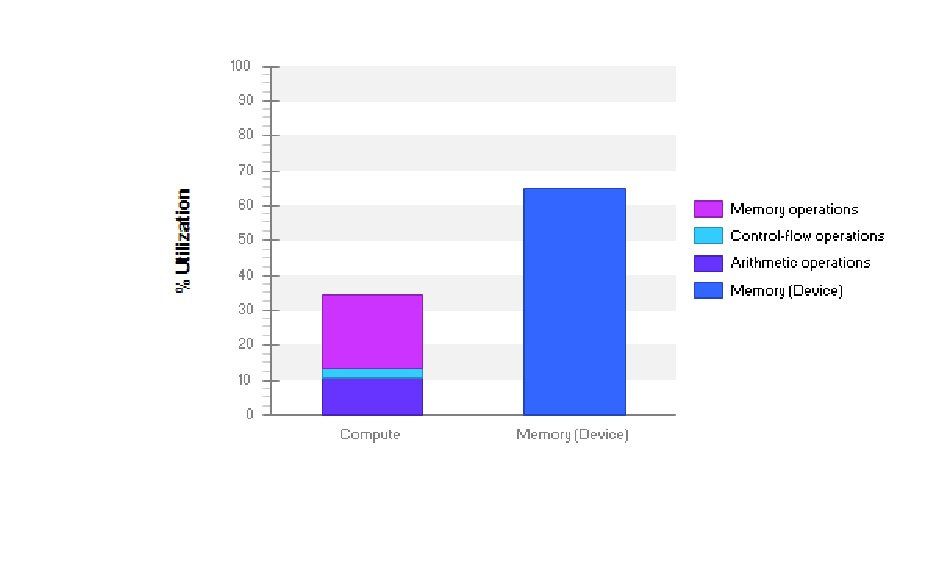
\includegraphics{utilization_histogram_small}
    \caption{GPU Utilization Histogram for smaller strings}
    \label{fig:}
  \end{center}
\end{figure}
\newline
The \textit{figure 5.2} can be explained as follows:
If the string size is less, the amount of ALU computation is less as compared to memory intensive operations whose initial startup overhead is high.Control-Flow operations occupy a very less \% of utilization as we had optimised the code to reduce the branches to virtually just one branch.
\begin{figure}
  \begin{center}
    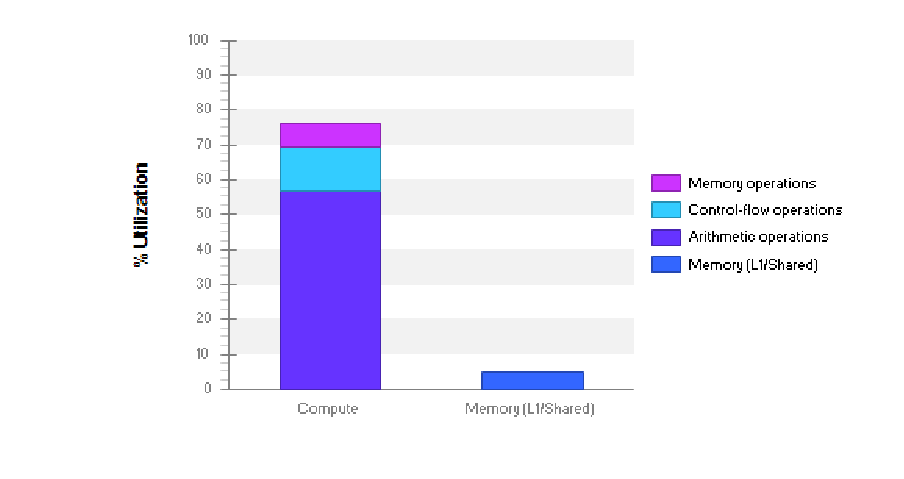
\includegraphics{utilization_histogram_large}
    \caption{GPU Utilization Histogram for larger strings}
    \label{fig:}
  \end{center}
\end{figure}
\newline
The \textit{figure 5.3} can be explained as follows:
As the string size increases, the amount of ALU computation increases more as compared to the increase in memory intensive operations. Thus, we see now that ALU Computation comprises more utilization \% to that of Memory Operations.

\subsection{Resource Utilisation}
Different types of instructions are executed on different functions on each SM. Performance can be limited if a function unit is over-used by the instructions executed by the kernel (refer \textit{figure 5.4}). The following result show that the kernel's performance is not limited by overuse of any function unit.
\newline
The four function units are:
\begin{itemize}
  \item Load/Store
  \item Arithmetic
  \item Control Flow
  \item Texture
\end{itemize}
\begin{figure}
  \begin{center}
    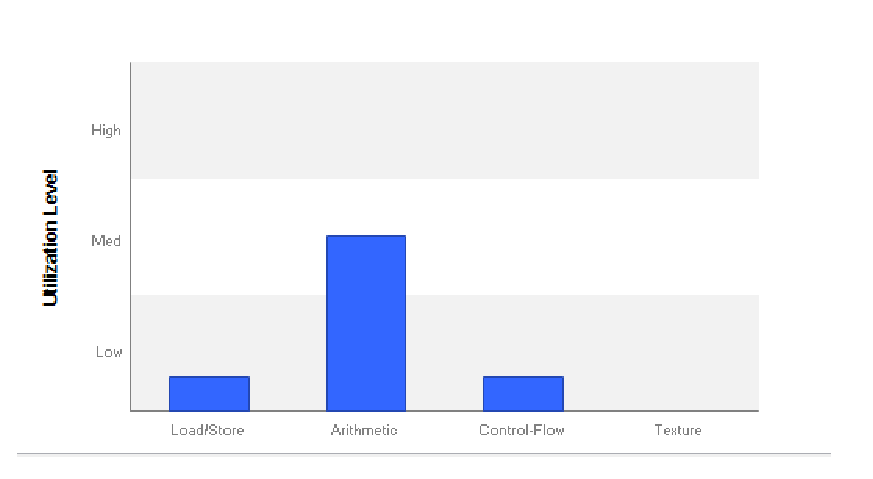
\includegraphics{utilization_functional}
    \caption{Functional Utilization}
    \label{fig:}
  \end{center}
\end{figure}
\subsection{Memory Bandwidth}
Validating observations:
\newline
We observe that global load transactions are approximately thrice the global store transactions (refer \textit{figure 5.5}). This should have been the case since in our algorithm at each step we read three elements to compute the minimum and store them at a particular position.
Moreover the bandwidth for global store is 10 times less than that of global load and thus even though we have less number of stores, they may be suspected to be the bottleneck.
 \begin{figure}
   \begin{center}
     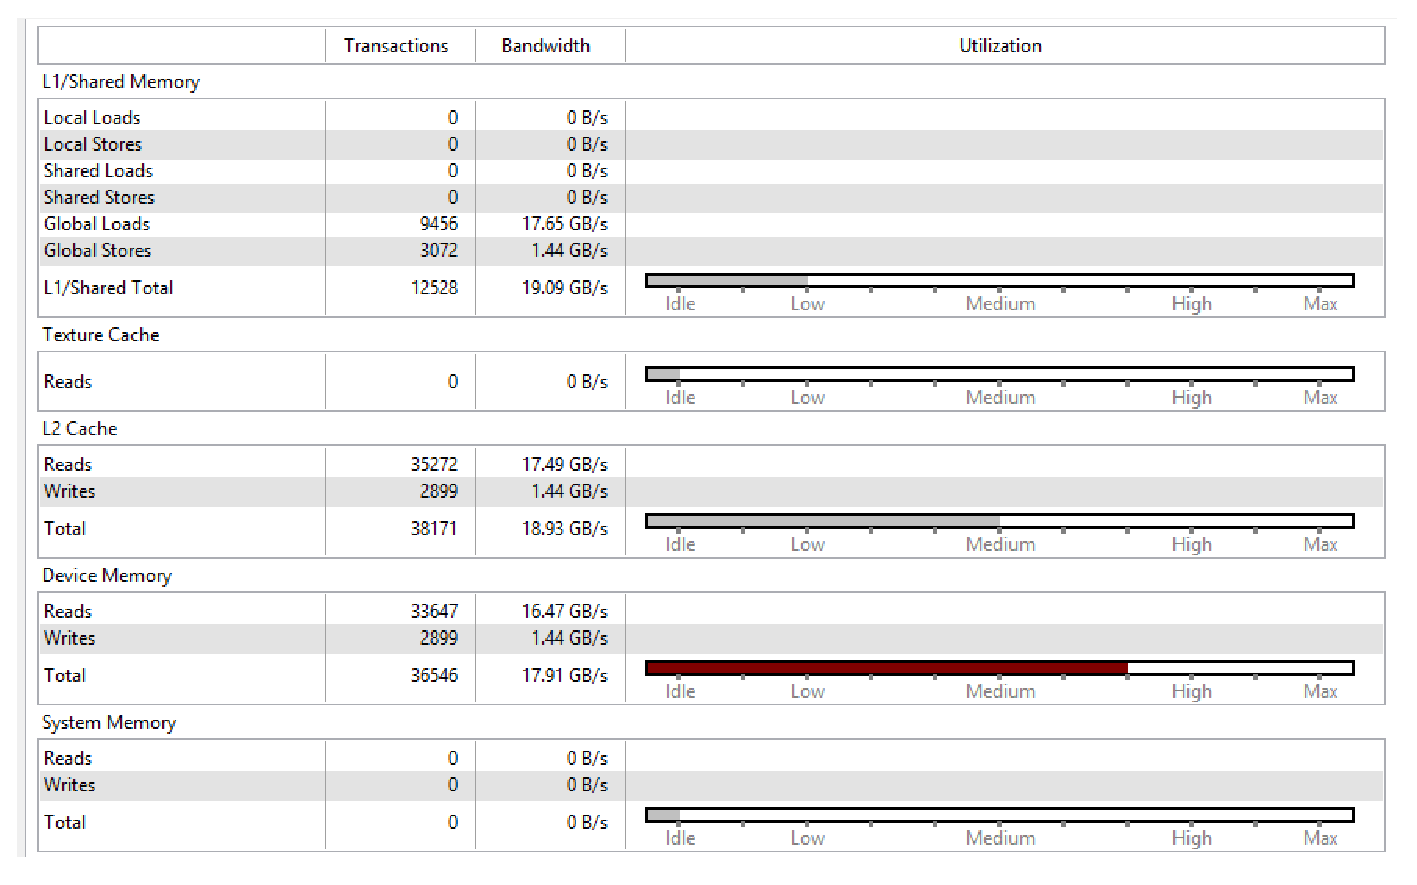
\includegraphics[width=15cm]{utilization}
     \caption{Bandwidth Utilization}
     \label{fig:}
   \end{center}
 \end{figure}
 
\subsection{Metrics}
\begin{itemize}
  \item Low Memory / Compute Overlap: The \% of the time memcpy is performed in parallel with compute is low.
  \item Low Memory Copy Throughput: Memory copies are not fully utilizing the host to device bandwidth. We are copying very less data from host to device but a signicantly large amount of data from device to host. For instance PCI express bus transfers data at a rate higher than 500MB/s but we are copying data in the order of only a few kilobytes from host to device and hence are not able to reach the potential.
    \item Low Global Memory Load/Store Efficiency: Since the computation is alu intensive poor access patterns leading to inefficient use of global memory bandwidth.
    
\end{itemize}
\chapter{Conclusion}
From our experiments, we observed that on increasing the string length above 18000 characters we get exception of CUDA Memory exceeded, this implies that we have reached the maximum possible potential of our implementation. But with GPU's with higher device memory we can align significantly large strings.\\ \newline
Also if the original problem consisted of finding only the magnitude of the alignment and not the exact string alignment, we could modify our algorithm which could work on strings much higher in length because in this case, we would be needing only a linear amount of space. \\ \newline
Overall GPU can significantly cut down the computation time and thus can have wide application in computing sequence alignment for real life problems.
\chapter{Acknowledgement}
\begin{itemize}
  \item Prof. Bernard Menezes, for teaching and encouraging us to work on GPU's.
  \item Prof. Sharath Chandran, for guiding us towards our problem statment.
  \item Ms. Lorin Ahmed, for her constant and timely help during the complete duration of the project.
\end{itemize}
\section{Softwares}
\begin{itemize}
  \item{Visual Studio, Microsoft } 
  \item{Compute Unified Device Architecture 5.5, NIVIDIA}
\end{itemize}
\end{document}
